	\documentclass[11pt,a4paper]{article}
\usepackage[utf8]{inputenc}
\usepackage{amsmath}
\usepackage{amsfonts}
\usepackage{graphicx}
\usepackage[table,xcdraw]{xcolor}


\usepackage{caption}
\usepackage{subcaption}

\renewcommand{\familydefault}{\sfdefault} % cambiamos la fuente a una sans

\usepackage{float} % para que floten las imagenes o algo asi...
\usepackage{wallpaper} %paquete para usar una imagen como encabezado!
\usepackage{hyperref} %para usar hypervinculos 
\usepackage[export]{adjustbox} %para usar marcos en imagenes
\usepackage{eurosym} % para el euro
\usepackage{transparent} %para las marcas de agua
\usepackage{eso-pic}  %para las marcas de agua
\definecolor{azul_marcos}{RGB}{0,128,159} %defino el color azul de los marcos
\usepackage{sectsty} %esto es para cambiar el color de las fuentes creo
\renewcommand{\familydefault}{\sfdefault} % cambiamos la fuente a una sans
\sectionfont{\color{azul_marcos}}  % sets colour of sections
\subsectionfont{\color{azul_marcos}}  % sets colour of sections


\usepackage{pdfpages} %para insertar pdfs
\usepackage{amssymb}
\usepackage{pstcol} % para color
\usepackage{pst-node} % para diagramas
\usepackage{pst-plot} % para representacion de dat
\usepackage[spanish]{babel}
\addto\captionsspanish{\renewcommand\chaptername{Bloque}}
%\usepackage[total={18cm,21cm},top=2cm, left=2cm]{geometry}
\usepackage{anysize}
\pagestyle{plain}
%\markboth{left head}{right head}
%\markright{Guía de impresión FlexiSMART}
\marginsize{3cm}{2cm}{2.5cm}{1cm}
\title{Guía de impresión Baobab}
\date{}

%configuracion de la marca de agua
\AddToShipoutPicture{
    \put(0,0){
        \parbox[b][\paperheight]{\paperwidth}{%
            \vfill
            \centering
            {\transparent{0.2}
\includegraphics[scale=1.25]{FOTOS/logofff}}%
            \vfill
        }
    }
}

\begin{document}
\ULCornerWallPaper{1}{FOTOS/header}
\LLCornerWallPaper{1}{FOTOS/footer}
%\maketitle
%\tableofcontents

\includepdf{PDF/ES_PORTADA.pdf}
\section{¿Qué es Baobab?}Baobab es un filamento para impresión 3D FFF/FDM que incorpora partículas de madera para imprimir objetos que imitan a la madera. 
\begin{figure}[H]
\centering
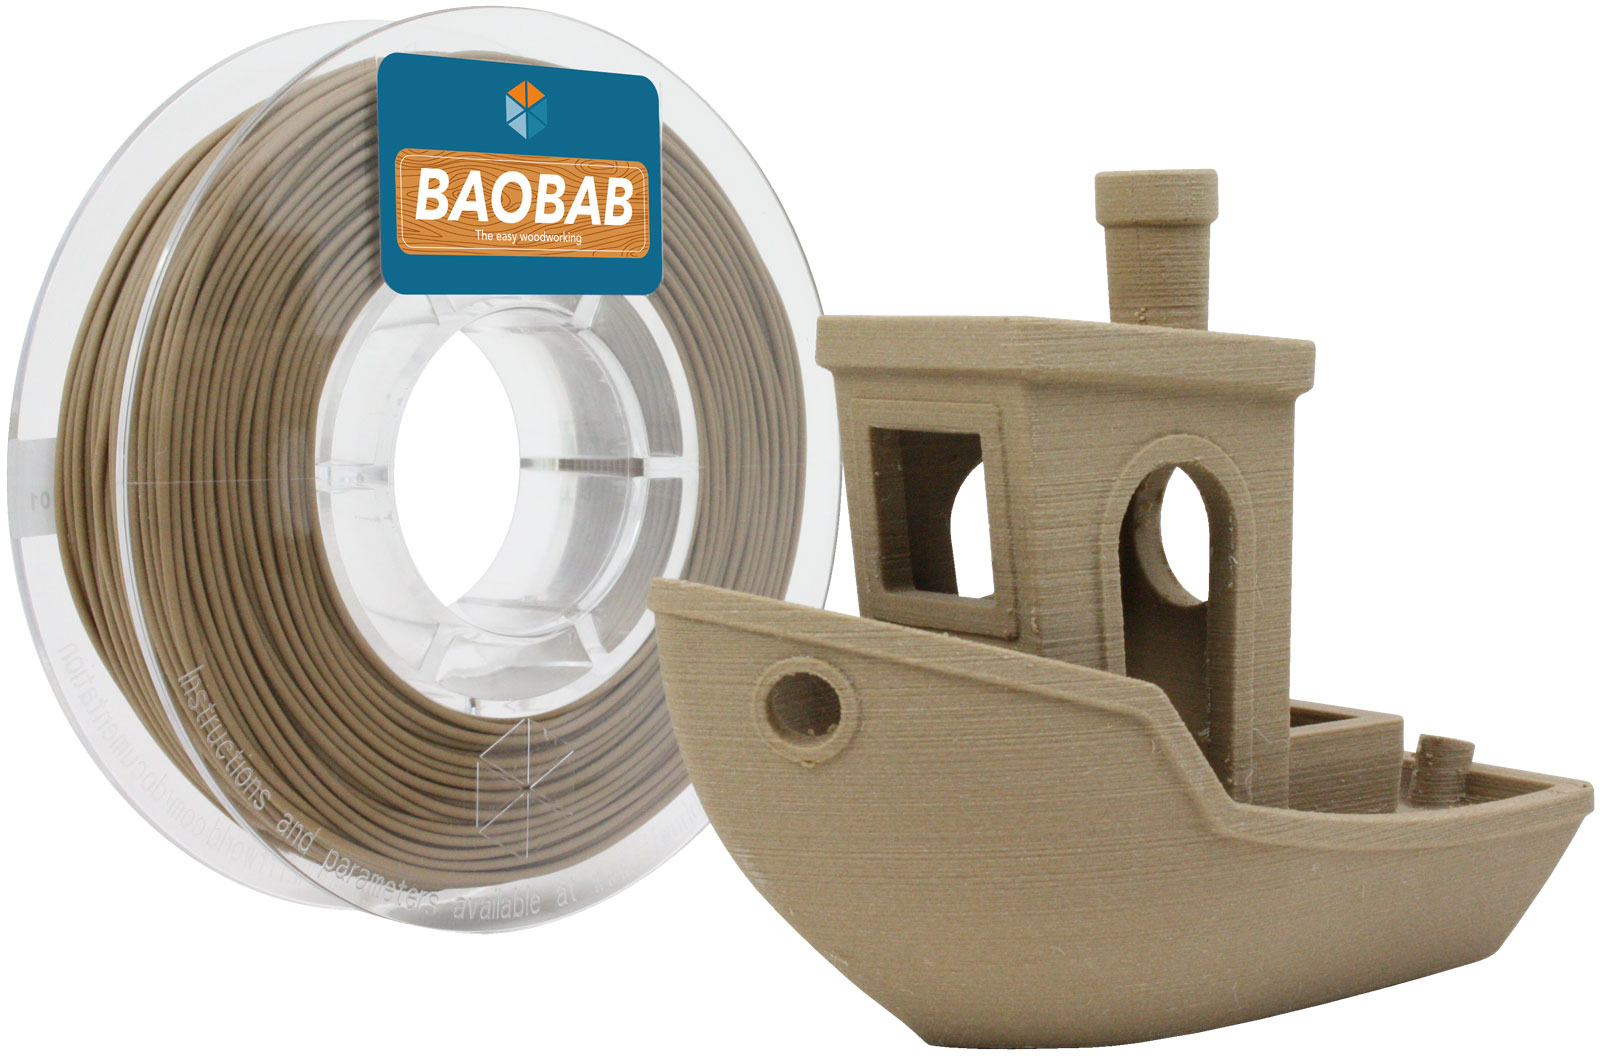
\includegraphics[width=0.6\textwidth,cfbox=azul_marcos 4pt 0pt]{FOTOS/BAOBAB_3DBENCHY}
\caption*{Baobab, filamento con base PLA con partículas de madera}
\end{figure}
\section{¿Por qué usar Baobab?}
Baobab permite crear objetos con apariencia de madera utilizando una impresora 3D. Es un material ideal para imprimir piezas que por su naturaleza o destino se beneficien de tener un aspecto similar a la madera.\\\\
Es un filamento ideal para crear esculturas, apliques, elementos de carpintería, etc.. También puede utilizarse en tareas de restauración.\begin{figure}[H]
\centering
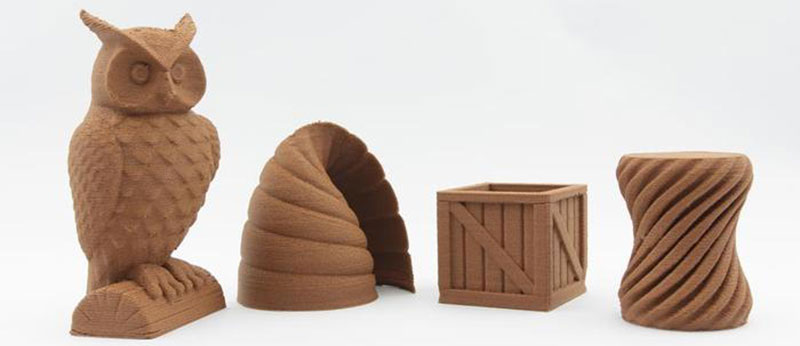
\includegraphics[width=1\textwidth,cfbox=azul_marcos 4pt 0pt]{FOTOS/SAMPLE_PARTS}
	\caption*{Ejemplos de piezas impresas}
\end{figure}
Baobab es compatible con la mayoría de impresoras 3D FFF/FDM ya que no necesita cama caliente y se imprime a una temperatura similar al PLA.\\\\
Al incorporar partículas de madera no fusibles la resistencia es inferior a la del PLA, pero es en general suficiente para la mayoría de aplicaciones típicas.\\\\
Baobab no sufre de efecto warping y permite imprimir piezas de gran volumen sin temor a que sufran deformaciones al enfriarse.
\section{Ficha técnica y parámetros de impresión}
\begin{table}[H]
\centering
\caption*{Ficha técnica}
\begin{tabular}{|
>{\columncolor[HTML]{FFFFFF}}l |
>{\columncolor[HTML]{FFFFFF}}c |}
\hline
\multicolumn{1}{|c|}{\cellcolor[HTML]{FFFFFF}\textbf{Material}}   & PLA con partículas de madera   \\ \hline
	\textbf{Densidad}                         & 0.93 g/cm3      \\ \hline
	\textbf{Temperatura de deflexión térmica}                         & 70ºc      \\ \hline
	\textbf{Temperatura de fusión}                         & 160ºc      \\ \hline
	\textbf{Temperatura de descomposicion}                         & \textgreater 270º c      \\ \hline
	\textbf{Elongación máxima}                         & 40\%      \\ \hline
\end{tabular}
\end{table}
\begin{table}[H]
\centering
\caption*{Parámetros de impresión recomendados}
\begin{tabular}{|
>{\columncolor[HTML]{FFFFFF}}l |
>{\columncolor[HTML]{FFFFFF}}c |}
\hline
\multicolumn{1}{|l|}{\cellcolor[HTML]{FFFFFF}\textbf{Diámetro de nozzle recomendado}} & 0.6 mm              \\ \hline
	\textbf{Temperatura recomendada (hot-end)}                         & 200ºc      \\ \hline
	\textbf{Temperatura recomendada (cama caliente)}                         & 40º - No necesita      \\ \hline
	\textbf{Velocidad recomendada de impresión}                         & 80 mm/s      \\ \hline
	\textbf{Distancia de retracción}                         & Depende del hot-end (Entre 4 y 20 mm)      \\ \hline
	\textbf{Velocidad de retracción}                         & La máxima soportada (Entre 50 y 100 mm/s)      \\ \hline
\end{tabular}
\end{table}
Puedes descargarte nuestros perfiles completos de impresión de los principales programas de laminación (Cura, Slic3r y Simplify3D) desde nuestra página web:\\\\
\centerline{ {\huge \url{www.fffworld.com/documentation} } }
\\\\
Los parámetros óptimos dependerán de la impresora 3D que utilices, sin embargo, son unos buenos parámetros para tenerlos como punto de partida. Con unas pocas impresiones serás capaz de encontrar los lmites y la configuración perfecta para tu maquina.
\section{Problemas y soluciones}
	\subsection{Entendiendo el problema}
Para conseguir un aspecto similar a la madera este filamento incorpora partículas de madera real. El tamaño y la cantidad de estas partículas está estudiado para evitar atascos pero aún así en algunas impresoras y bajo determinadas circunstancias los atascos pueden producirse y estropear la impresión.\\\\
Los atascos pueden surgir por dos causas diferenciadas y en dos puntos diferentes del hot-end: el nozzle y el barrel. En caso de aparecer, es necesario identificar la causa para ponerle solución e imprimir satisfactoriamente.\begin{figure}[H]
\centering
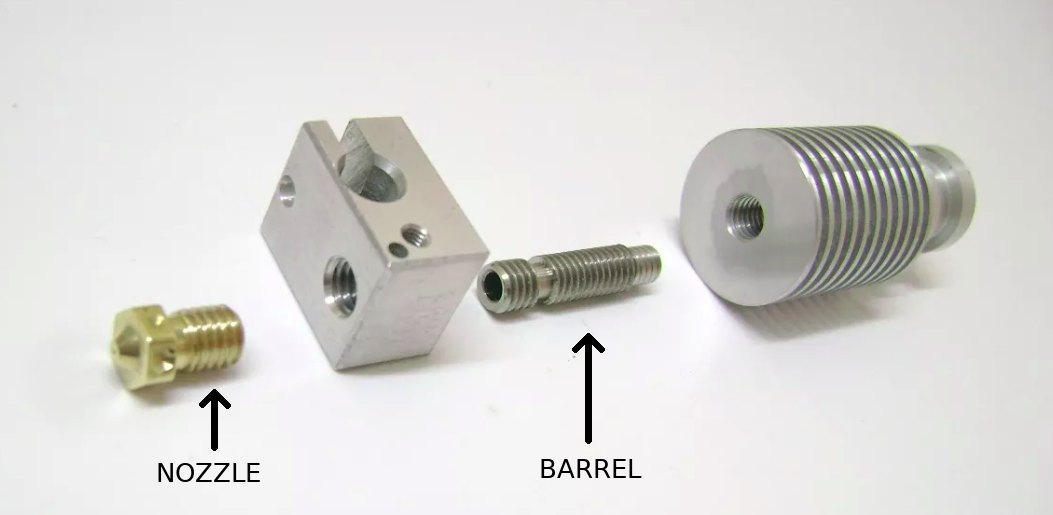
\includegraphics[width=0.8\textwidth,cfbox=azul_marcos 4pt 0pt]{FOTOS/BARREL_AND_NOZZLE}
\caption*{Hot-end E3D desmontando}
\end{figure}
		\subsubsection{Atascos en el nozzle}
Los atascos en el nozzle se producen por acumulación de partículas de madera en la boquilla. La madera no se funde, como sí lo hace el plástico, y puede acumularse en el nozzle durante la impresión provocando un atasco.\begin{figure}[H]
\centering
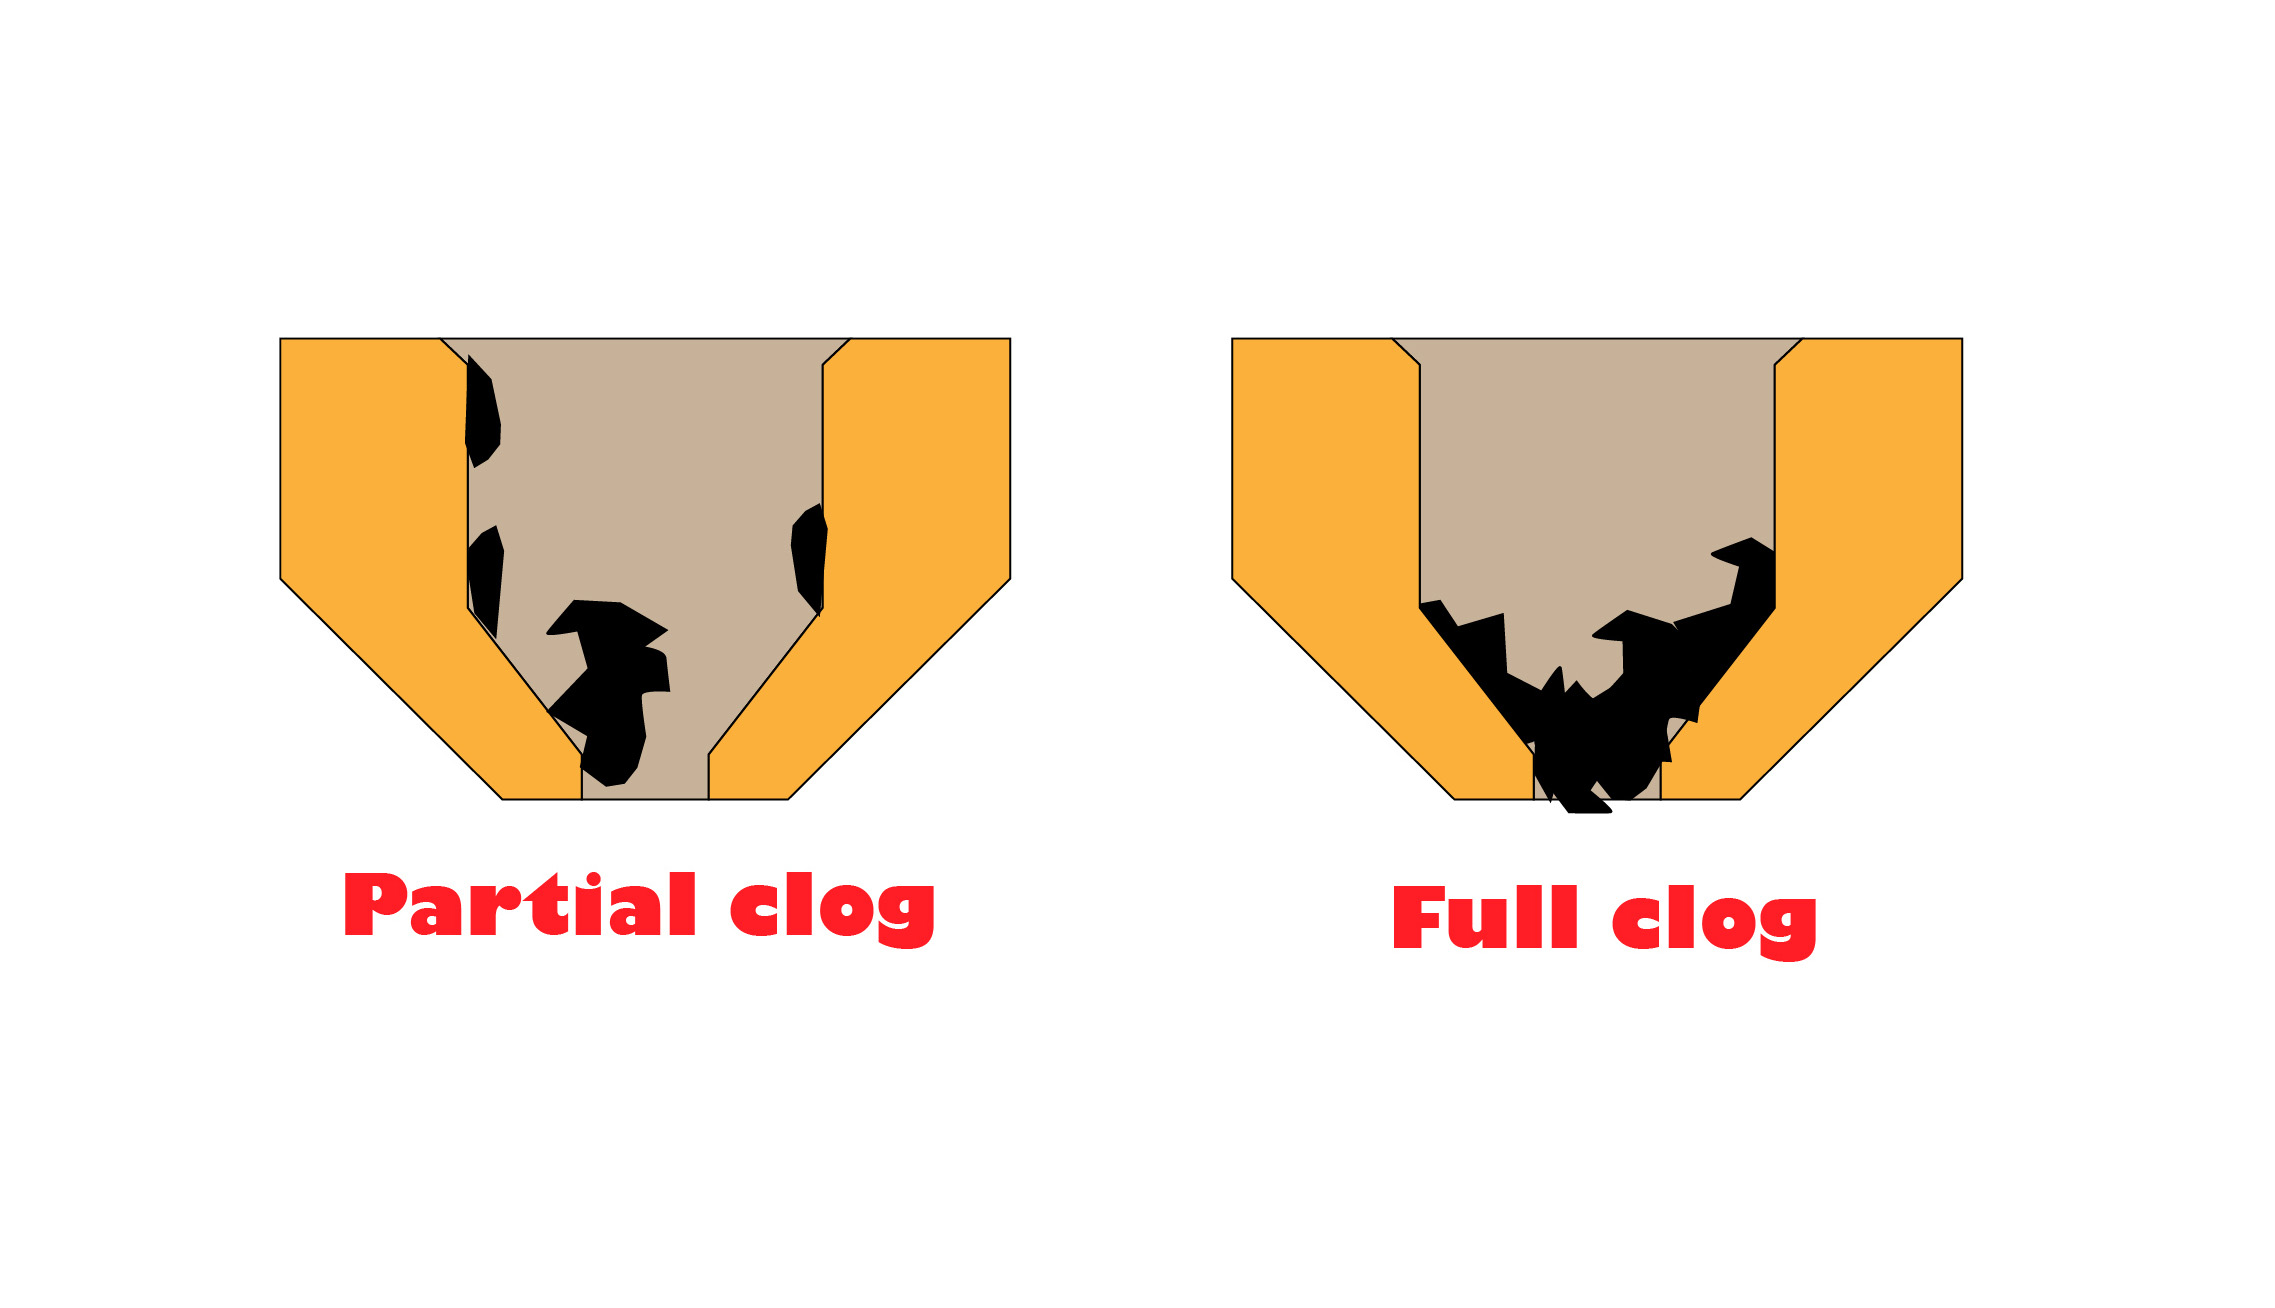
\includegraphics[width=0.5\textwidth,cfbox=azul_marcos 4pt 0pt]{FOTOS/NOZZLE_CLOG}
\caption*{Comparación entre atasco parcial y total del nozzle}
\end{figure}
El tamaño del nozzle, la calidad del mismo, el material del que está hecho y la presencia de restos de otros materiales son determinantes en la aparición de atascos en el nozzle.\\\\
Si se están produciendo atascos en el nozzle la mejor solución es utilizar un nozzle diámetro superior. Utilizando un nozzle de 0.6 mm el problema desaparece en la mayoría de los casos.\\\\
En nuestra tienda online podrá encontrar el nozzle que mejor se adapte a su impresora. Además si compra filamento Baobab le ofrecemos un descuento en la compra de nozzles.		\subsubsection{Atascos en el barrel}
Estos atascos se producen por la expansión que sufre el filamento al calentarse. Al tener una superficie rugosa, debido a su contenido de madera, el filamento Baobab produce un mayor rozamiento en las paredes internas del barrel o puente térmico.\begin{figure}[H]
\centering
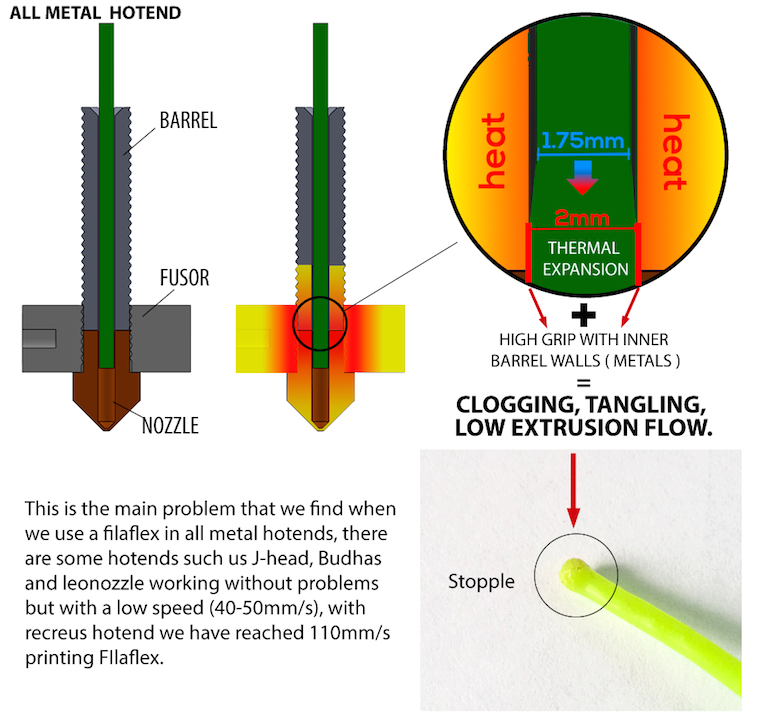
\includegraphics[width=0.5\textwidth,cfbox=azul_marcos 4pt 0pt]{FOTOS/EXPANSION}
\caption*{Esquema de los atascos en el barrel causados por la expansión del filamento}
\end{figure}
Este rozamiento produce atascos y problemas de extrusión en algunos hot-ends, especialmente en aquellos con mala refrigeración, sin tubo de teflón en su interior o con un mecanizado de baja calidad.%FOTO BARREL
	\subsection{Controlando la retracción}
Los atascos en el barrel pueden controlarse modificando los parámetros de retracción. Los parámetros de retracción adecuados dependen de cada hot-end, pero la idea general es hacer retracciones largas y rápidas para evitar que el extremo del filamento permanezca en la zona más caliente del barrel cuando no está siendo extruido. De esta manera cuando el hot-end se desplaza entre 2 puntos sin extruir, la punta del filamento permanece en una zona fría, evitando la expansión.\\\\
Le recomendamos que pruebe los siguientes rangos de retracción en caso de que tenga problemas de atascos:	\begin{description}
		\item[Velocidad de retracción:] La máxima soportada por su impresora. Este valor puede estar entre 50 y 100 mm/s 
		\item[Distancia de retracción:] Lo ideal es medir la distancia que hay entre el nozzle y la zona fría del hot-end. Esta distancia puede ser de entre 4 mm. y 20 mm. dependiendo del hot-end 
	\end{description}
\begin{figure}[H]
\centering
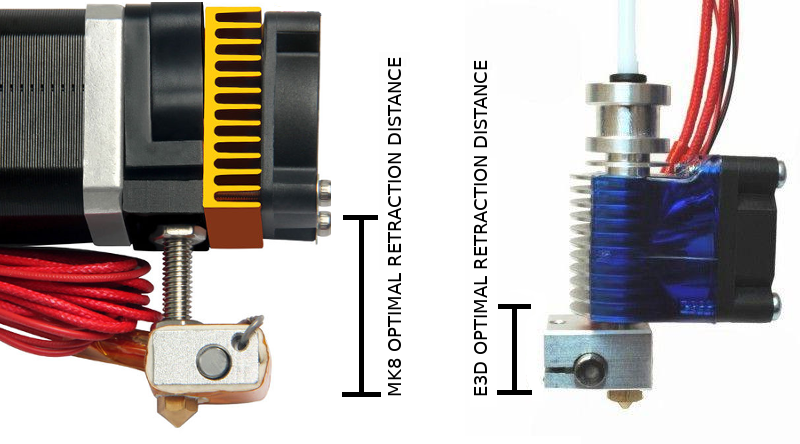
\includegraphics[width=0.8\textwidth,cfbox=azul_marcos 4pt 0pt]{FOTOS/RETRACTION}
\caption*{La distancia óptima de retracción hay que medirla para cada hot-end}
\end{figure}
	\subsection{Aumentando la velocidad}
Otra estrategia que ayuda a evitar estos problemas es aumentar la velocidad de impresión, con el objetivo de dar menos tiempo al filamento a expandirse y atascar potencialmente en el barrel.\\\\
La velocidad máxima depende de cada impresora pero una velocidad de 80 mm/s suele ser adecuada para reducir estos atascos.	\subsection{Mejorando la refrigeración del hot-end}
Los problemas mencionados tienen su origen en una refrigeración pobre del hot-end. \\\\
Utilizando un hot-end con una buena refrigeración, como por ejemplo un E3D original, que incorpora un disipador y un ventilador apuntando directamente al mismo, estos atascos no deben producirse.\begin{figure}[H]
    \centering
    \begin{subfigure}[b]{0.4\textwidth}
        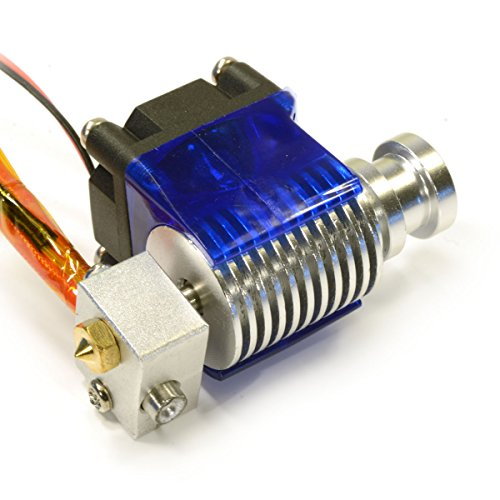
\includegraphics[width=\textwidth,cfbox=azul_marcos 4pt 0pt]{FOTOS/E3D_GOOD_COOLING}
		\caption*{Hot-end E3D con disipador y ventilador refrigerando directamente el barrel}
    \end{subfigure}
    ~ \qquad%add desired spacing between images, e. g. ~, \quad, \qquad, \hfill etc. 
      %(or a blank line to force the subfigure onto a new line)
    \begin{subfigure}[b]{0.4\textwidth}
        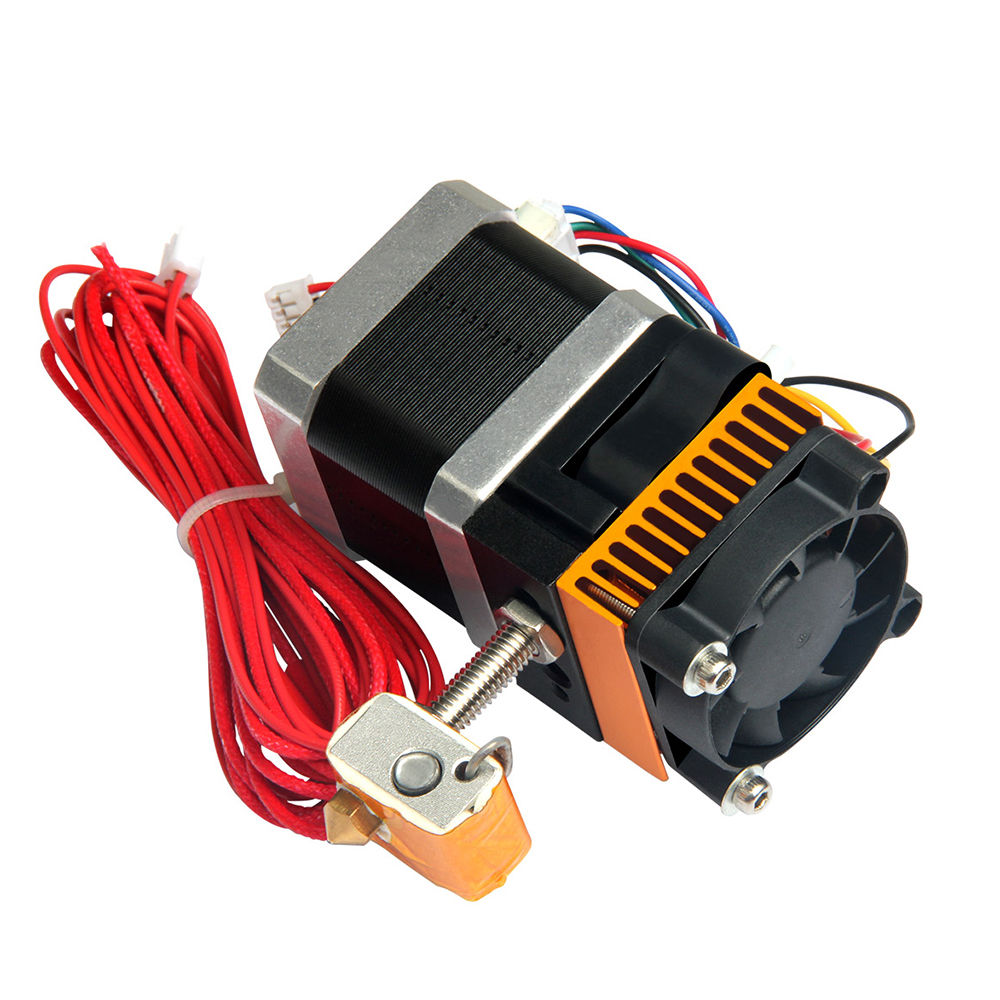
\includegraphics[width=\textwidth,cfbox=azul_marcos 4pt 0pt]{FOTOS/MK8_BAD_COOLING}
		\caption*{Extrusor MK8 con mucha distancia de barrel y sin refrigeración directa}
    \end{subfigure}
\end{figure}
Colocar un ventilador extra o dirigir el flujo de aire hacia el barrel, reduce la expansión del filamento y puede solucionar completamente los atascos.\\\\
En páginas como thingiverse pueden encontrarse accesorios imprimibles para distintos modelos de hot-ends e impresoras que permiten acoplar un ventilador y mejorando la refrigeración.\\\\
Otras soluciones menos elegantes pero efectivas pasan por utilizar bridas o modificar la posición del ventilador existente de manera que el flujo de aire incida directamente en el barrel del hot-end. Está opción puede ser adecuada para testar la solución de manera rápida antes de aventurarse a imprimir e instalar un accesorio como los mencionados anteriormente.\begin{figure}[H]
    \centering
    \begin{subfigure}[b]{0.4\textwidth}
        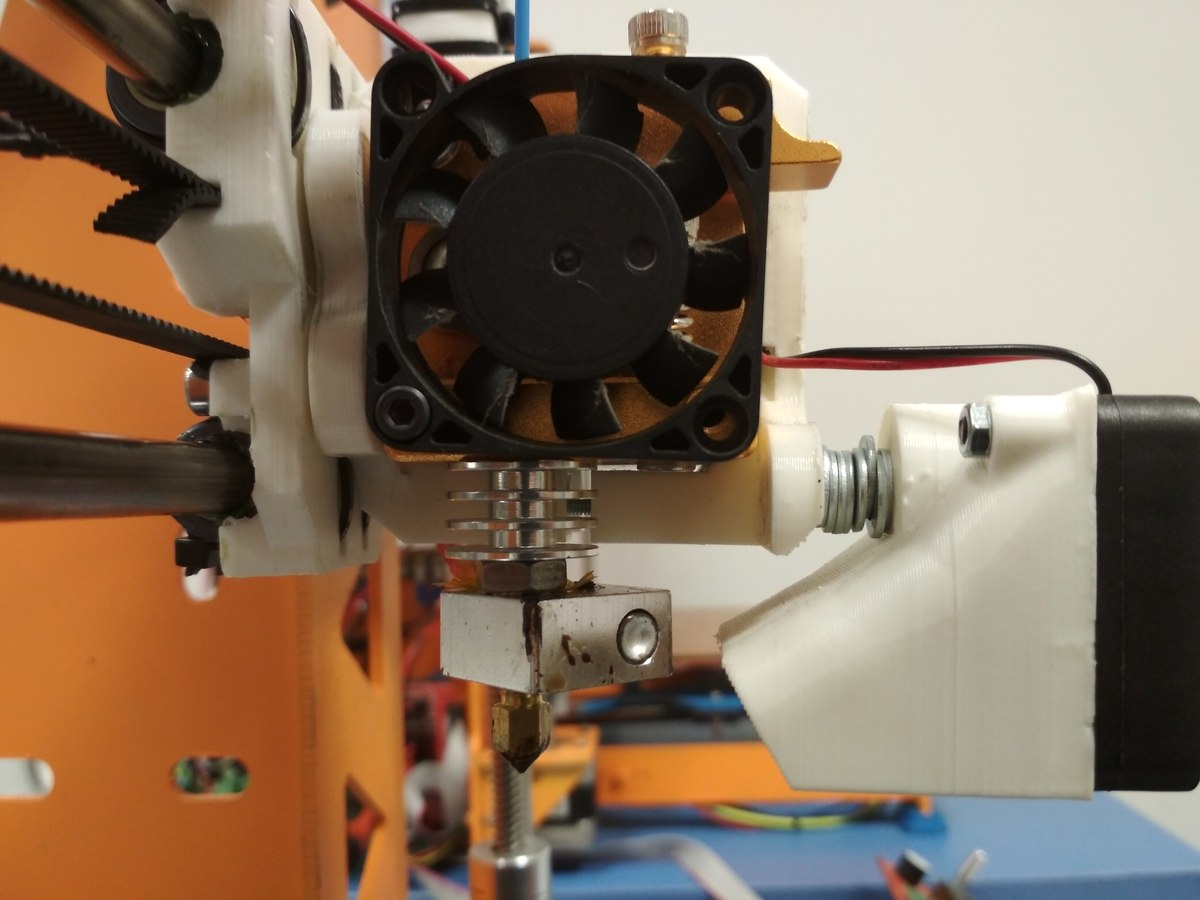
\includegraphics[width=\textwidth,cfbox=azul_marcos 4pt 0pt]{FOTOS/MK8_FAN_TRICK1}
		\caption*{Posición original del ventilador en el extrusor MK8}
    \end{subfigure}
    ~ \qquad%add desired spacing between images, e. g. ~, \quad, \qquad, \hfill etc. 
      %(or a blank line to force the subfigure onto a new line)
    \begin{subfigure}[b]{0.4\textwidth}
        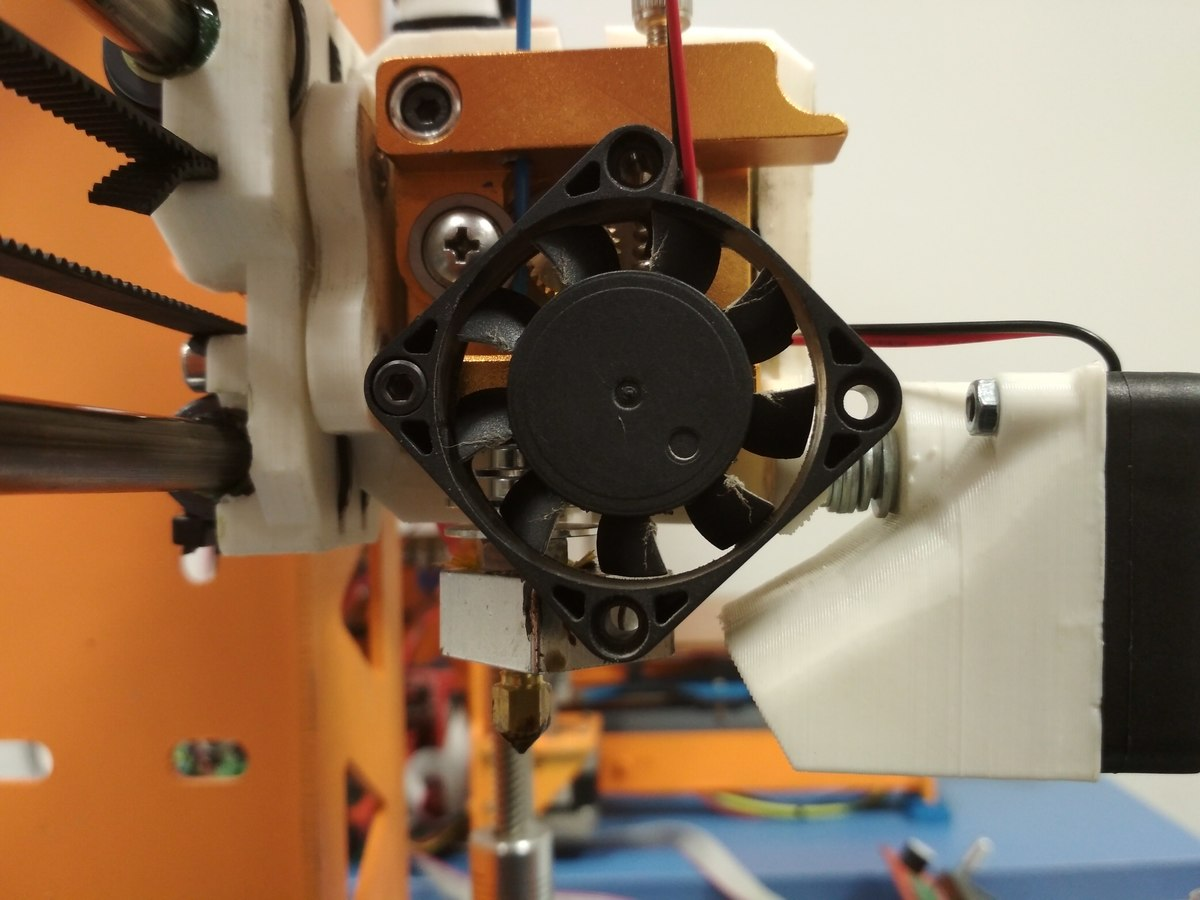
\includegraphics[width=\textwidth,cfbox=azul_marcos 4pt 0pt]{FOTOS/MK8_FAN_TRICK2}
		\caption*{Ventilador girado para apuntar directamente al barrel}
    \end{subfigure}
\end{figure}
	\subsection{He sufrido un atasco ¿ahora qué?}
Cuando se produce un atasco la extrusión se interrumpe y si no se detiene la impresión y se enfría el hot-end, puede producirse una degradación del material en su interior que empeore la situación.\\\\
Esto sucede porque al dejar de extruir, el filamento queda inmóvil en el interior del hot-end a temperatura de impresión. Al permanecer calientes demasiado tiempo, los plásticos se cristalizan y carbonizan haciendo que el atasco sea más difícil de eliminar.\\\\
Podemos saber si hay material carbonizado en el interior del nozzle si resulta imposible extruir manualmente el material aplicando una fuerza moderada.\\\\
Afortunadamente los atascos de Baobab, incluso cuando el material se ha degradado, son relativamente fáciles de eliminar utilizando las herramientas adecuadas.	\subsubsection{Desatascando el orificio del nozzle}
Introducir un elemento metálico por la boquilla desde la parte inferior es el primer paso para eliminar un atasco.\\\\
FFF world tiene a disposición de sus clientes agujas metálicas flexibles que resultan idóneas para este cometido, pero cualquier elemento metálico, lo suficientemente resistente como para no partirse, puede servirnos. En caso de no disponer de una de estas agujas, puede utilizar una cerda metálica arrancada previamente de un cepillo.\begin{figure}[H]
\centering
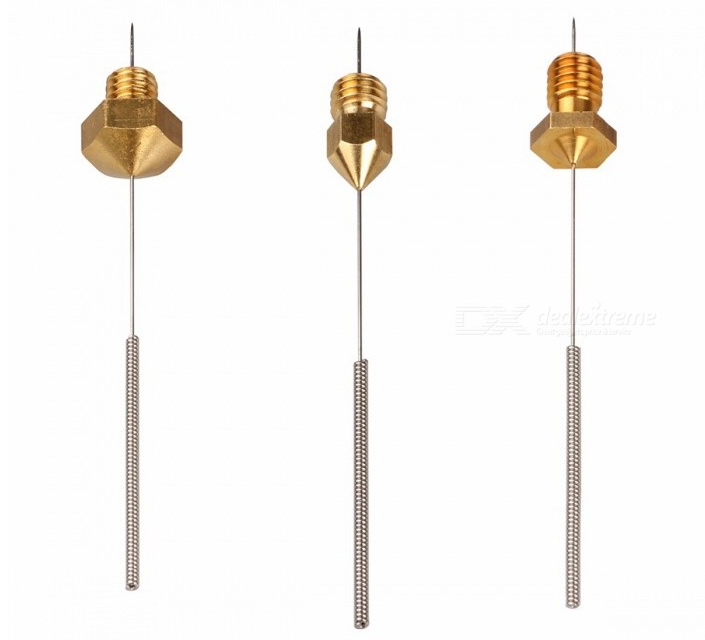
\includegraphics[width=0.4\textwidth,cfbox=azul_marcos 4pt 0pt]{FOTOS/NEDDLE}
\caption*{Aguja limpia nozzle}
\end{figure}
Con el hot-end caliente, introduzca la aguja por el orificio del nozzle en diferentes ángulos para eliminar los restos de filamento. Empuje manualmente el filamento desde la parte superior para comprobar si el atasco ha desaparecido. Repetir la operación hasta que el material fluya con normalidad.\begin{figure}[H]
    \centering
    \begin{subfigure}[b]{0.45\textwidth}
        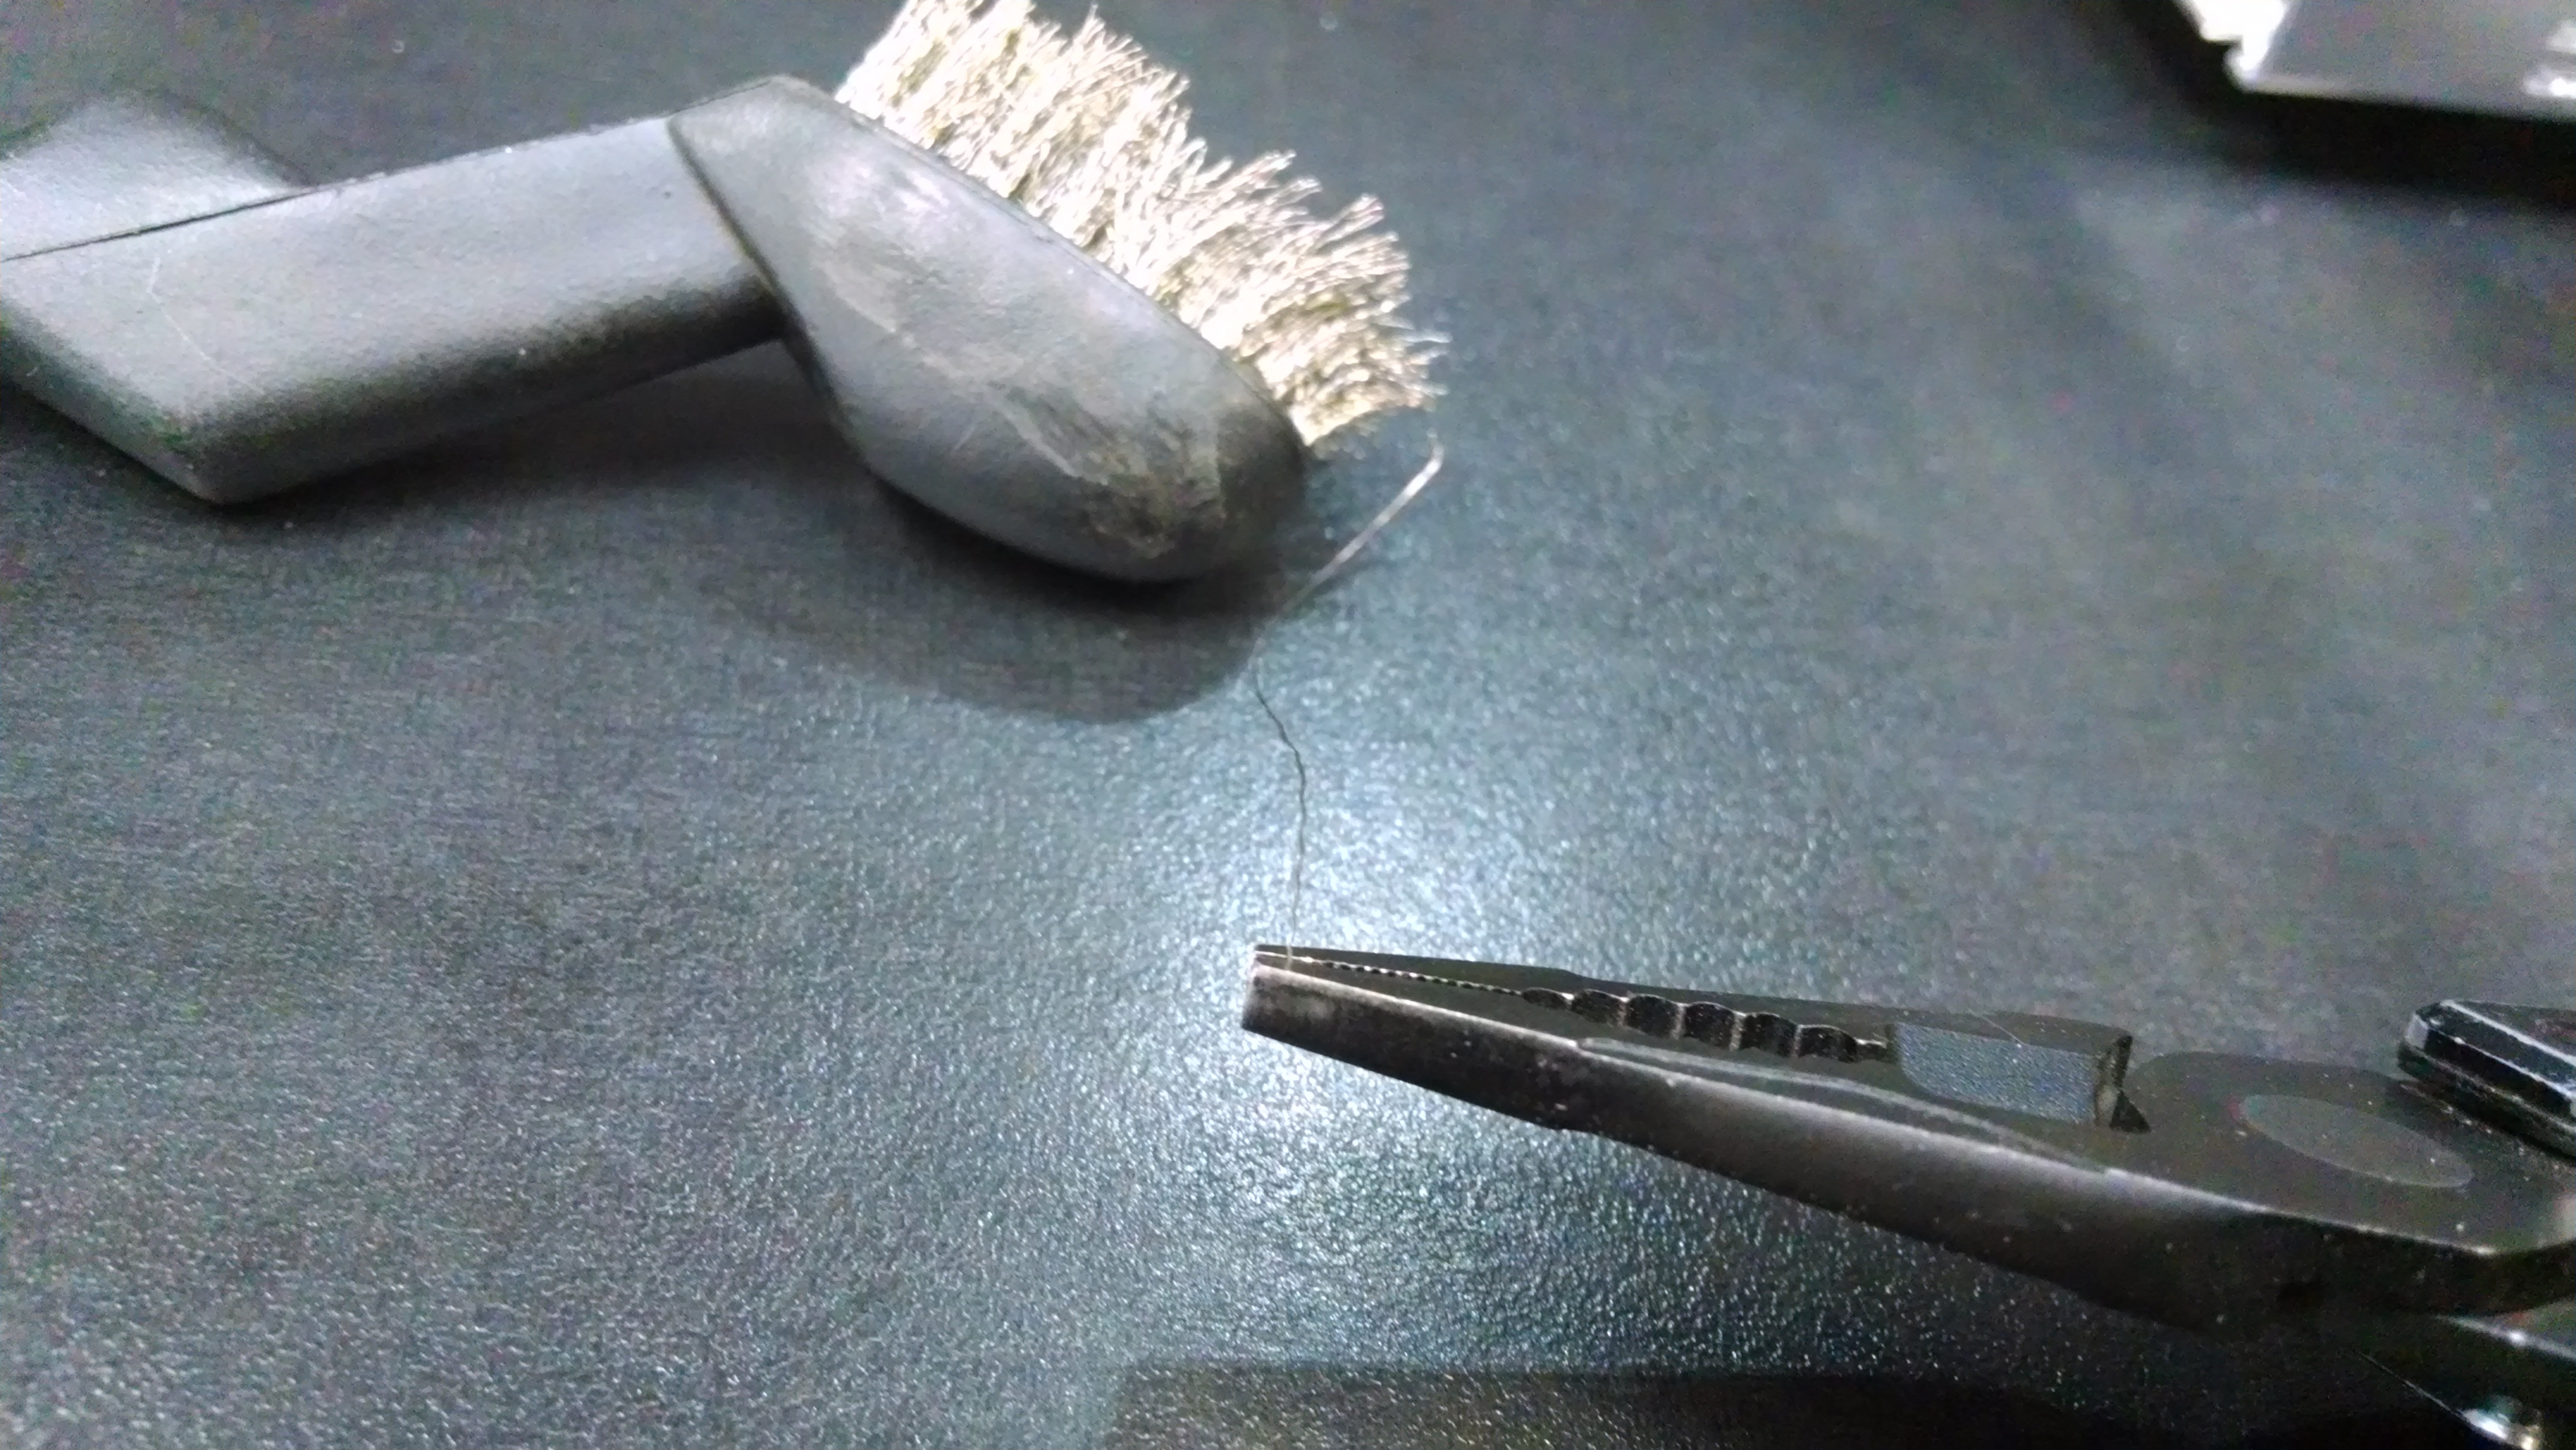
\includegraphics[width=\textwidth,cfbox=azul_marcos 4pt 0pt]{FOTOS/CEPILLO1}
    \end{subfigure}
    ~ %add desired spacing between images, e. g. ~, \quad, \qquad, \hfill etc. 
    \quad
      %(or a blank line to force the subfigure onto a new line)
    \begin{subfigure}[b]{0.45\textwidth}
        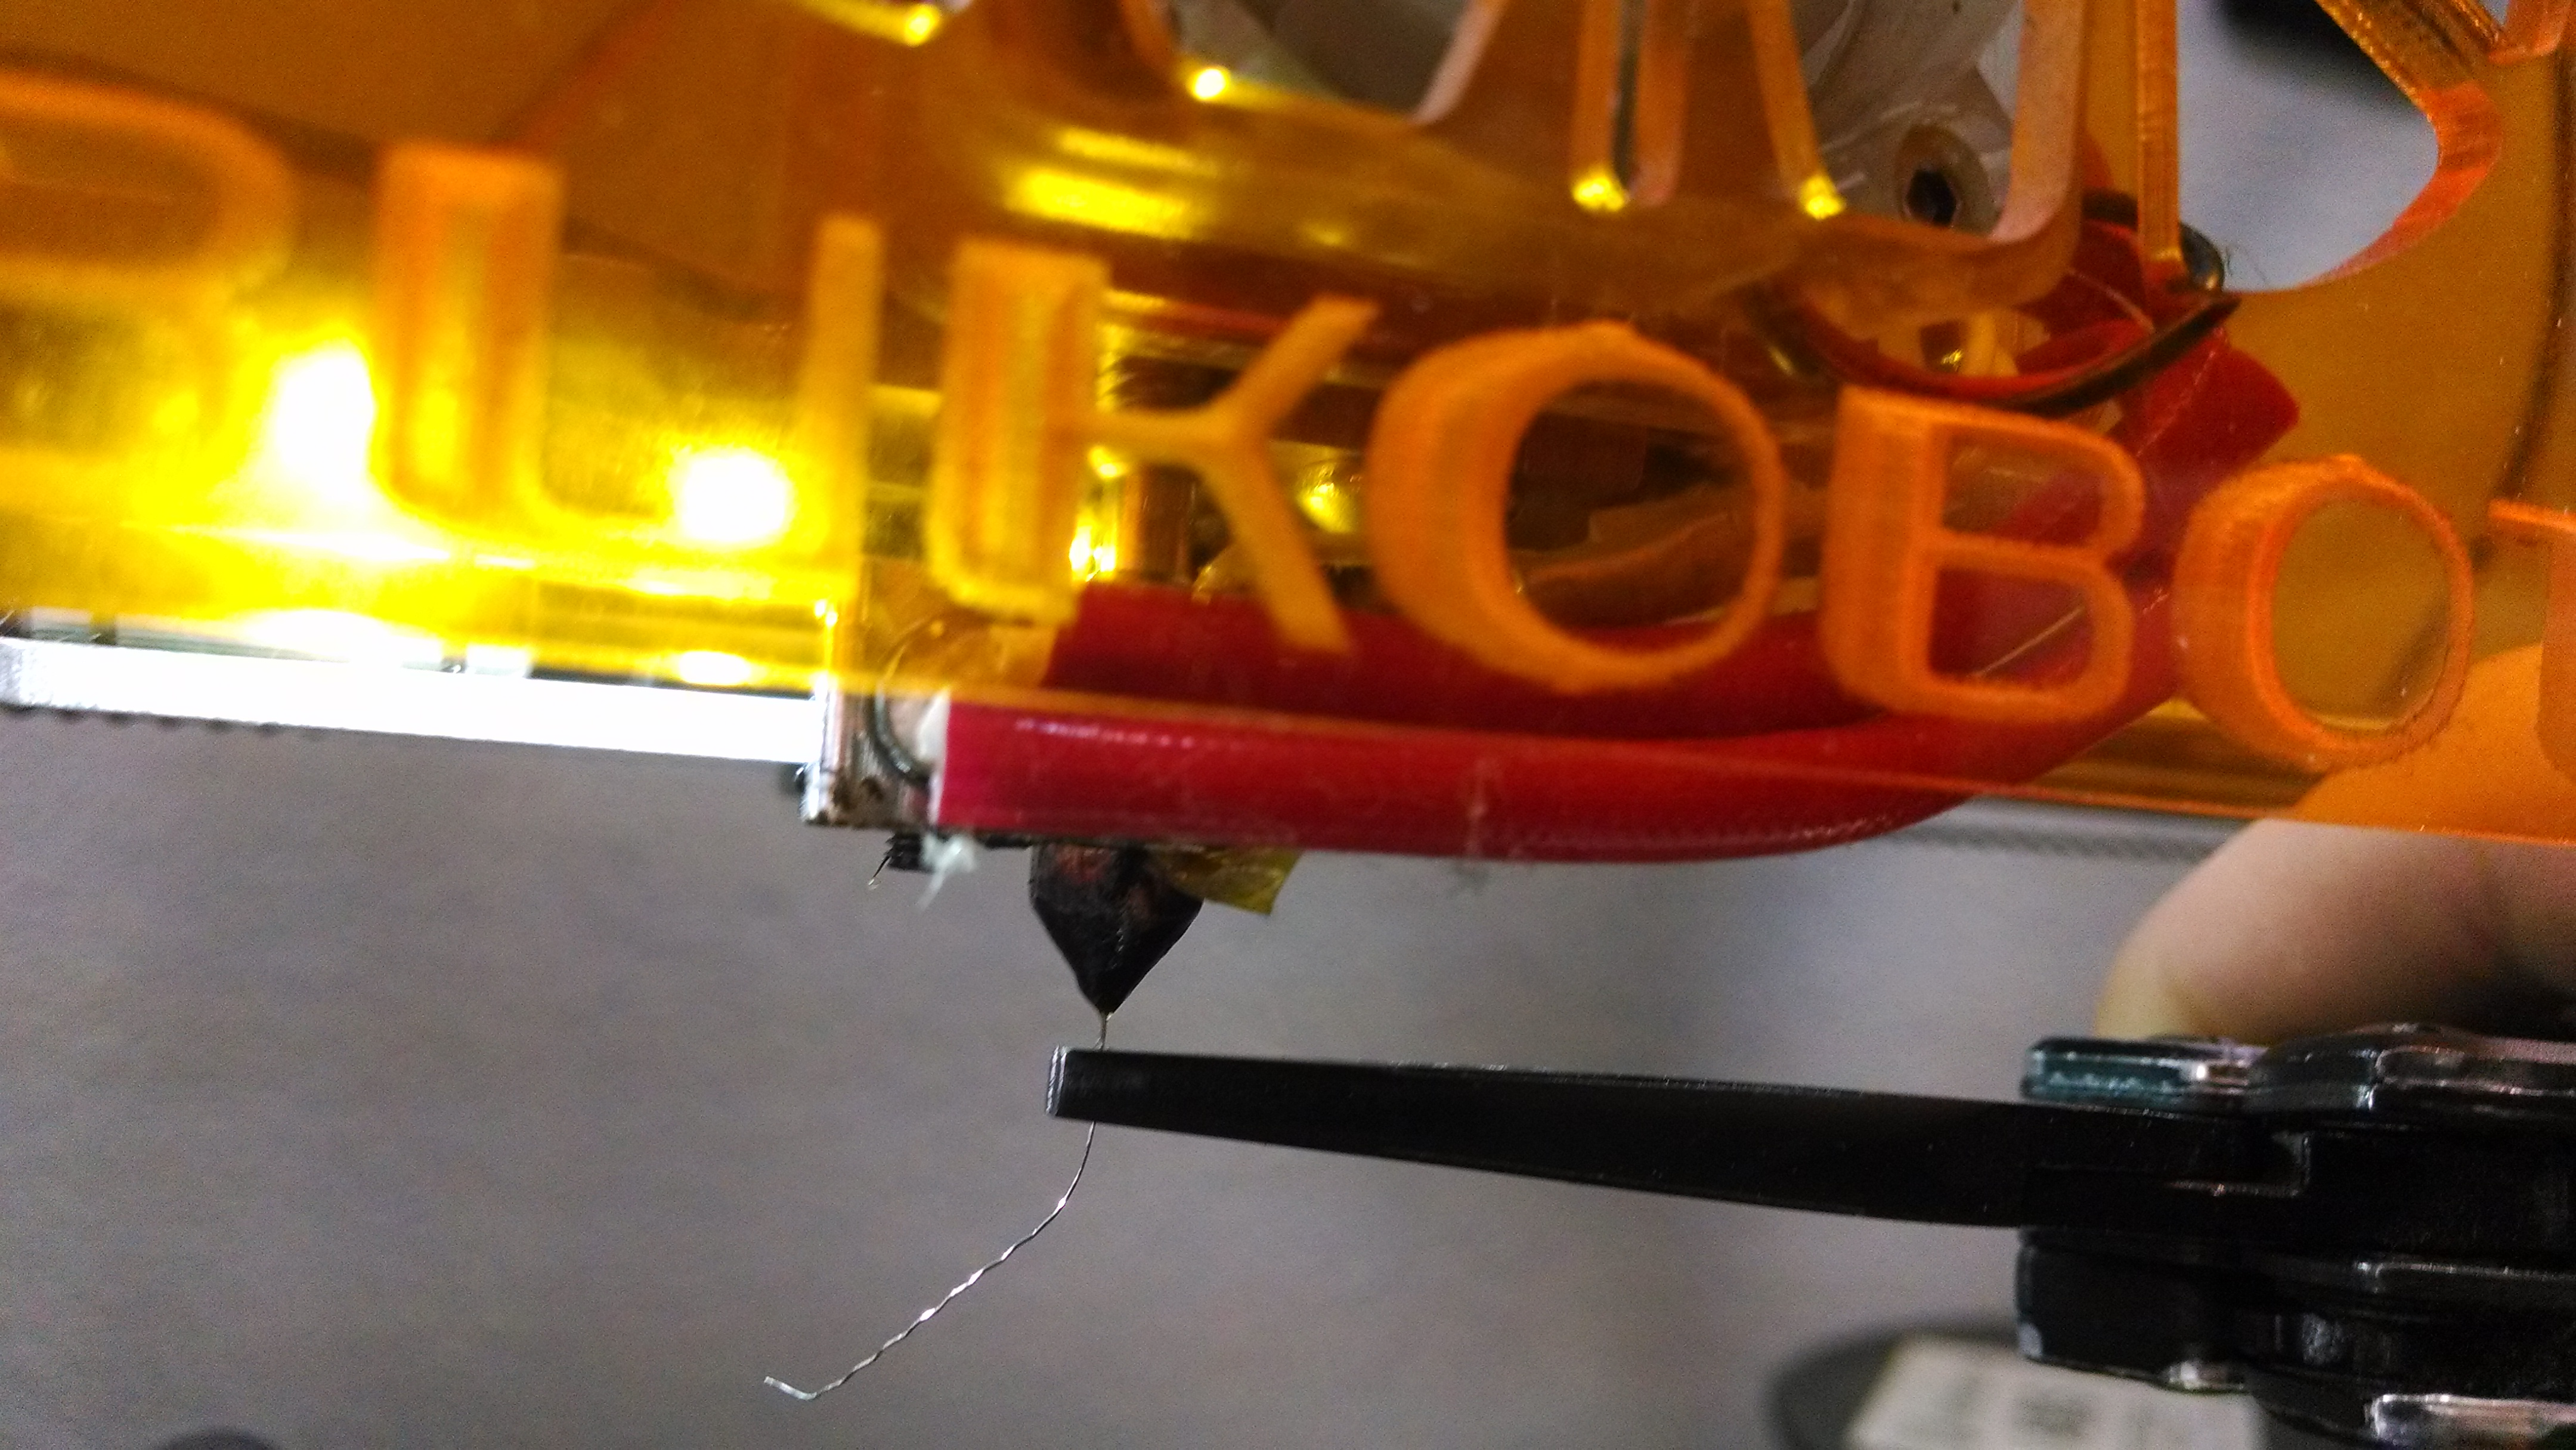
\includegraphics[width=\textwidth,cfbox=azul_marcos 4pt 0pt]{FOTOS/CEPILLO2}
    \end{subfigure}
    \caption*{Utilización de una hebra metálica para limpiar el nozzle}
\end{figure}
	\subsubsection{El método cold pulling o tirón en frío.}
Éste método bautizado consiste en tratar de extraer los restos de filamento desde la parte superior del hot-end, utilizando otro trozo de filamento.\\\\
Para ello se caliente el hot-end a la temperatura del último material usado y se introduce un trozo de filamento por la parte superior del hot-end hasta que salga por el nozzle o no podamos empujarlo más. El filamento introducido se fundirá y quedará pegado a los restos de material en el interior del hot-end. En ese momento, se baja la temperatura a 90º en el caso del Baobab o del PLA (o 110º si se trata de ABS) y se tira del filamento introducido con la intención de que al extraerlo se extraigan también los restos de material que producían el atasco.\begin{figure}[H]
\centering
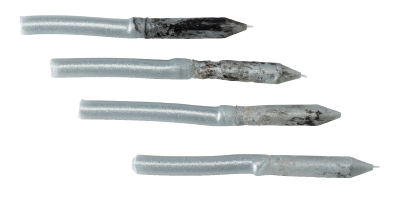
\includegraphics[width=0.6\textwidth,cfbox=azul_marcos 4pt 0pt]{FOTOS/COLD_PULLING}
\caption*{Repetir la operación hasta que el filamento salga limpio}
\end{figure}
Cada vez que repitamos la operación el filamento extraído debería salir más limpio. Repetir el proceso hasta eliminar el atasco completamente.\\\\
Puede leer más sobre el cold pulling en estos links: \\\\
\url{https://www.antonmansson.com/how-to-cold-pull-clogged-nozzle/}\\
\url{https://www.trideus.be/en/blogs/stories/tips-tricks-do-the-cold-pull/}\\
\url{https://ultimaker.com/en/resources/19510-how-to-apply-atomic-method}\\
\url{https://printrbot.zendesk.com/hc/en-us/articles/202100554-Unclogging-the-Hot-End-Using-the-Cold-Pull-Method}
	\subsubsection{Desmontando el nozzle}
Si todo lo demás falla la solución pasa por desmontar el nozzle.\\\\
Para ello es necesario calentar el hot-end y desenroscar el nozzle con una llave inglesa o una llave de tubo. Una vez desmontado debería ser sencillo eliminar los restos de material que puedan quedar en el barrel.\\\\
Una vez separado del hot-end, el nozzle se puede calentar con una pistola de aire caliente o en una vitrocerámica para eliminar completamente los restos de material.\\\\
Introducir el nozzle en acetona eliminará completamente el atasco si se trata de ABS . En el caso de Baobab o PLA, la acetona no disuelve el material pero también ayuda a limpiar el nozzle.\section{¿Quieres apoyar nuestro proyecto?}
Todos los miembros FFF World amamos la impresión 3D y la comunidad maker. Nos sentimos afortunados de poder trabajar en proyectos donde podamos entregar nuestra pasión sincera. En el futuro, nos gustaría poder desarrollar más materiales, más colores, más formatos. En definitiva, nos gustaría poder hacer crecer nuestra empresa.\\\\
Para ello, una de las principales acciones para ayudarnos, si quieres hacerlo y estás satisfecho con el filamento, es la de votarnos en Amazon con 5 estrellas.\begin{figure}[H]
\centering

\includegraphics[width=0.5\textwidth,cfbox=azul_marcos 1pt 0pt]{FOTOS/AMAZON_FIVE_STARS}
\caption*{¡Muchas gracias!}
\end{figure}
\subsection{Another filaments with outstanding properties available now in Amazon}
\begin{description}
\item[FlexiSMART Tech:] Diseñado para resistir a la abrasión y al desgaste de impresiones técnicas. 
\item[ABS Tech:] Efecto warping minimizado. Alto rendimiento en aplicaciones técnicas. 
\item[PETG Tech:] Máxima resistencia mécanica. Resistente al contacto con el agua y los rayos UV. Apto para uso alimentario. 
\item[FilaMETAL:] PLA con carga metálica no abrasiva que da un acabado metálico espectacular a tus impresiones. 
\item[PC Tech:] Policarbonato con gran resistencia a la temperatura y con excelentes propiedades mecánicas. 
\item[Nylon Tech:] Imprimible a baja temperatura. Resistencia a los golpes con cierto grado de flexibilidad. 
\item[PVA Tech:] Filamento soluble en agua indicado para uso como material de soporte. Excelente compatibilidad con PLA. 
\item[HIPS Tech:] Filamento soluble en limoneno indicado para uso como material de soporte. Buena resistencia mecánica y excelente compatibilidad con ABS. 
\end{description}

\includepdf{PDF/ES_CONTRAPORTADA.pdf}
\end{document}
